En esta sección, se busca resolver el problema de CMF a partir de una Heurística de Búsqueda Tabú (Tabu search\footnote{Glover, F. "Tabu Search — Part I", ORSA Journal on Computing 1989}). Dicha heurística consiste en una estrategia para resolver problemas combinatorios, aplicable tanto en grafos como en otras estructuras utilizadas para resolver problemas de lógica. Este método utiliza el mismo procedimiento que Búsqueda Local\footnote{Ver sección anterior.} para acercarse progresivamente a una mejor solución dentro de un entorno. Dado que en ciertos casos la solución no puede ser mejorada, la técnica de Búsqueda Tabú permite empeorarla parcialmente para proseguir la búsqueda de una mejor. A su vez, esta heurística concede una estructura llamada $lista\ tabú$ con distintas utilidades. Principalmente, sirve para guardar movimientos de modo a no repetirlos y/o guardar características o soluciones, entre otras. A continuación, se encuentra explicitado el pseudocódigo\footnote{http://www.dc.uba.ar/materias/aed3/2013/2c/laboratorio/heuristicas.pdf} de la heurística de Búsqueda Tabú:

\begin{algorithm}[H]
\SetAlgoLined
s$_{0}$ $\leftarrow$ solucion inicial \\
s$^{*}$ $\leftarrow$ s$_{0}$ \\
T $\leftarrow$ lista tabú inicial \\
\While{ no se alcance el criterio de terminacion}{
N $\leftarrow$ vecinos de s no tabú o mejores que s$^{*}$ \\
s $\leftarrow$ mejor solucion en N. \\
\If{ s es mejor que s$^{*}$}
 {s$^{*}$ $\leftarrow$ s} 
Actualizar la lista tabú T }
\end{algorithm}

\subsection{Explicación del algoritmo realizado}

 El algoritmo realizado parte de un valor entero positivo ingresado como parámetro, $desviacion\_permitida$, y de una solución provista por la Heurística de Búsqueda Local. A partir de esta última, el algoritmo busca, paulatinamente, una mejor solución siguiendo las siguientes opciones:
\begin{itemize}
 \item Agregando un nodo: Dada la solución actual (una clique), procede a $agregar$ un nodo que la mejore, es decir, que aumente su frontera.
 \item Quitando un nodo: Dada la solución actual (una clique), procede a $quitar$ un nodo que la mejore, es decir, que aumente su frontera.
\end{itemize}
A diferencia de la Búsqueda Local, se buscan nuevas soluciones que no necesariamente mejoren la solución obtenida hasta el momento pero que sí lo hagan a largo plazo. Sin embargo, dentro de las formas de empeorar la solución, se toma aquella que empeora lo menos posible. A su vez, a medida que se agrega o quita un nodo, se lo inserta en la lista tabú. Esto se realiza sin olvidar que siempre que pueda subir lo va a hacer, entonces, si descendiendo se encuentra con que puede volver a ascender, lo va a hacer hasta volver a estar en un máximo local.\newline

\begin{figure}[H] %[h] Aqui [b] para button [t] para top
\begin{center}
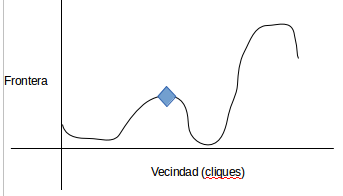
\includegraphics[width=250pt]{../imgs/1_tabu.png}
\caption{solución con Busqueda Local}
\end{center}
\end{figure}


\begin{figure}[H] %[h] Aqui [b] para button [t] para top
\begin{center}
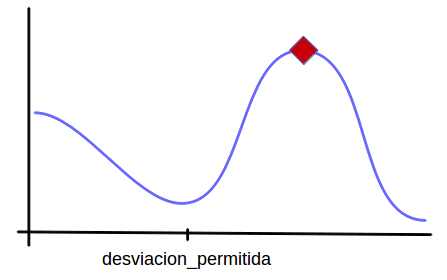
\includegraphics[width=250pt]{../imgs/2_tabu.png}
\caption{solución con Busqueda tabú}
\end{center}
\end{figure}

Al finalizar, el algoritmo retorna la mejor solución hallada. \newline

\textbf{Descripción de la lista tabú} \newline

 A medida que se van agregando o quitando nodos que no mejoran la solución, se los va marcando como tabú. De esta forma, se le asigna una prioridad a cada uno de ellos que depende del momento en que fue agregado. A su vez, sea cual sea la prioridad del último nodo insertado, éste no puede utilizarse en la iteración siguiente para evitar ciclar soluciones. Para lograr esto, hicimos que en el peor de los casos sólo se puedan usar los nodos tabús que tienen prioridad menor a la mitad de la prioridad máxima.\newline

\textbf{Criterio de terminación} \newline

 El algoritmo presentado tiene dos criterios de terminación. Por un lado, la cantidad de iteraciones en que la solución puede mejorar y, por el otro, la variable $desviacion\_permitida$ ingresada como parámetro. El primero se encuentra acotado por el máximo absoluto que existe pues el problema siempre tiene solución. Luego, pueden existir muchos máximos locales pero ninguno será una clique con mayor frontera que la del máximo absoluto (esto resulta trivial). Por otro lado, la variable $desviacion\_permitida$ va disminuyendo cada vez que se modifica la solución actual sin mejorarla, es decir, que permitimos avanzar de manera ``no creciente'' una cantidad $desviacion\_permitida$ de veces. \newline


\begin{algorithm}[H]
    \SetAlgoLined
    \caption{TabuSearch}
    \KwIn{\textbf{Conj(nodos)} $solución\_inicial$, \textbf{Grafo} $g$, \textbf{Entero} $desviacion\_permitida$}
    \KwOut{\textbf{Conj(nodos)} $solución\_final$}

	\textbf{Conj(nodos)} sol$_{0}$,sol$_{1}$ \\ 
	\textbf{Conj(nodos)} $solución\_actual$ $\leftarrow$ LocalSearch($solución\_inicial$, $g$)	\\	
	\textbf{Conj(nodos)} $solución\_final$ $\leftarrow$ $solución\_actual$	\\	
	\textbf{Lista Tabu} $\leftarrow$ $\{\}$\\
	\textbf{Boolean} $Mejore\ la\ frontera$ $\leftarrow$ true

	\While{ $Mejore\ la\ frontera$ $\vee$ 0 $<$ $desviacion\_permitida$}{

	 	sol$_{0}$ $\leftarrow$ Dame Mejor solución agregando nodo No Tabu ($solución\_inicial$,$solución\_final$) \\
		sol$_{1}$ $\leftarrow$ Dame Mejor solución quitando nodo No Tabu ($solución\_inicial$,$solución\_final$) \\
		\If{ frontera(sol$_{0}$) $<$ frontera(sol$_{1}$)}
			{sol$_{0}$ $\leftarrow$ sol$_{1}$}
		\eIf{ frontera($solución\_actual$) $<$ frontera(sol$_{1}$)}
			{$solución\_actual$ $\leftarrow$ sol$_{0}$ \\
			$Mejore\ la\ frontera$ $\leftarrow$ true
			}
			{$Mejore\ la\ frontera$ $\leftarrow$ false \\
			 Poner Tabu Nodo utilizado en sol$_{0}$ \\
			 $desviacion\_permitida$ - 1}
		$solución\_actual$ $\leftarrow$ sol$_{0}$ \\
		\If{ frontera($solución\_final$) $<$ frontera($solución\_actual$) } 
		{$solución\_final$ $\leftarrow$ $solución\_actual$}			
	}

    	\textbf{devolver} $solución\_final$ \\

\end{algorithm}

\begin{algorithm}[H]
    \SetAlgoLined
    \caption{Dame Mejor solución agregando nodo No Tabu}

	$solución\_final$ $\leftarrow$ $solución\_inicial$ con un nodo mas cualquiera \\
	\ForAll{$u \in Candidatos\_clique($solución\_inicial$)$}{
	 		\If{$u$ $\notin Nodos(solución\_inicial)$}{
				\eIf{$\neg$ es tabu($u$)}{
		 			\If{frontera($solución\_final$) $<$ frontera( $solución\_inicial$ con $u$) }{
						$solución\_final$ $\leftarrow$ $solución\_inicial$ con $u$}
				}{
					\If{ Es Tabu aceptable ($u$) $\land$ frontera($solución\_final$) $<$ frontera( $solución\_inicial$ con $u$)}
					{$solución\_final$ $\leftarrow$ $solución\_inicial$ con $u$}
				
				}
			}
	}

\end{algorithm}

\begin{algorithm}[H]
    \SetAlgoLined
    \caption{Dame Mejor solución quitando nodo No Tabu}

	$solución\_final$ $\leftarrow$ $solución\_inicial$ sin un nodo cualquiera \\
	\ForAll{$u \in$ Nodos($solución$\_$inicial$)}{
		\eIf{$\neg$ es tabu($u$)}{
	 		\If{frontera($solución\_final$) $<$ frontera( $solución\_inicial$ sin $u$)}{
	 			$solución\_final \leftarrow solución\_inicial$ sin $u$}
		}{
				\If{Es Tabu aceptable ($u$) $\land$ frontera($solución\_final$) $<$ frontera($solución\_inicial$ con $u$)}
					{$solución\_final$ $\leftarrow$ $solución\_inicial$ con $u$}
		}
	}

\end{algorithm}

Donde:
\begin{itemize}
 \item $desviacion\_permitida$ consiste en la cantidad de veces que se agrega o quita un nodo por iteración (empeorando la solución parcial).
 \item $frontera$ es una función que, dada una clique pasada como parámetro, devuelve su frontera.
 \item $Candidatos\_clique$ devuelve los nodos que pertenecen a la clique máxima a partir de un conjunto de éstos pasado como parámetro.
 \item $Nodos$ devuelve los nodos pertenecientes a la solución pasada como parámetro.
 \item $Es\ tabú\ aceptable$ verifica si la prioridad de un nodo perteneciente a la lista tabú es menor a la mitad de la prioridad máxima, en cuyo caso se define como aceptable.
\end{itemize}

\subsection{Complejidad Temporal}

 Para desarrollar la complejidad de este algoritmo, estudiemos las estructuras y las formas en las que se guardan los datos. \newline

 Cuando nos referimos a una ``solución'' en el código, nos referimos a una estructura ($solucionTabu$) que consiste en dos listas\footnote{http://www.cplusplus.com/reference/list/list/}, $adentro$ y $candidatos$, un vector $esta$ y un entero $cantFrontera$:
\begin{itemize}
 \item $adentro$: Lista que indica los nodos que contiene la solución actual.
 \item $candidato$: Lista de los nodos candidatos a formar una clique máxima (teniendo en cuenta los nodos de $adentro$). 
 \item $esta$: Vector booleano de nodos que están en la solución.
 \item $cantFrontera$: Entero que indica la frontera de la solución.\newline
\end{itemize}
 Como puede observarse, $adentro$, $candidato$ y $esta$ están acotados por la cantidad de nodos, $n$. De esta forma, copiar una solución consiste en copiar dichas estructuras, lo que resulta lineal respecto del tamaño. Luego, $\mathcal{O}(3^*n)$ = $\mathcal{O}(n)$.\newline 
 La función $cantFrontera$ calcula la frontera de una solución con complejidad temporal constante dado que retorna únicamente el elemento. A su vez, operaciones como agregar o quitar un nodo consisten en realizar los siguientes pasos: \newline
\begin{itemize}
 \item $Copiar\ una\ solución$ actual a una nueva (como ya vimos es lineal en la cantidad de nodos)
 \item $Quitar\ o\ agregar\ un\ nodo$ de $esta$ y $adentro$. Ponerlo como ausente en $esta$ es constante (es solo acceder al nodo) y eliminarlo de la lista es lineal en la cantidad de elementos a eliminar\footnote{http://www.cplusplus.com/reference/list/list/erase/}, pero como solo eliminamos uno, es constante. Por otro lado, agregar un elemento en $esta$ es constante (por el mismo argumento anterior) y agregarlo a la lista también lo es\footnote{http://www.cplusplus.com/reference/list/list/push\_back/}.
 \item $Calcular\ los\ candidatos$ donde borramos la lista anterior de candidatos\footnote{http://www.cplusplus.com/reference/list/list/clear/} (esto es lineal en la cant. de nodos en el peor caso) y luego se recorren todos los nodos, a su vez de todos los que estan en $adentro$ para ver adyacencias (esto tiene un costo de $\mathcal{O}(n)^{2}$) mientras que se va insertando los que corresponden\footnote{http://www.cplusplus.com/reference/list/list/push\_back/}.
 \item $Calcular\ la\ frontera$ consiste en recorrer los nodos de $adentro$ (lineal en cant. de nodos) y luego restarles la cantidad de nodos de la clique (que es $n*(n-1)$ con $n$=nodos de la clique)
\end{itemize}
 Siendo así que agregar o quitar un nodo tienen un costo de $\mathcal{O}(n)$ + $\mathcal{O}(1)$ + $\mathcal{O}(1)$ + $\mathcal{O}(n^2)$ + $\mathcal{O}(n)$ = $\mathcal{O}(n^2)$.\newline

 Por otro lado, la lista tabú esta representada por un vector de $n$ elementos donde en la i-esima posición esta el "valor tabú" del i-esimo nodo. Por lo tanto, poner como tabú a un nodo o ver su valor es equivalente a acceder\footnote{http://www.cplusplus.com/reference/vector/vector/operator[]/} a un elemento del arreglo que es constante.\newline

 Teniendo en cuenta todo lo anterior, empecemos viendo las complejidades de las funciones $Dame$ $Mejor$ $solución$ $agregando$ $nodo$ $No$ $tabú$ y $Dame$ $Mejor$ $solución$ $agregando$ $nodo$ $No$ $tabú$. Como se puede observar en los algoritmos ambas son son similares en cuanto a las operaciones realizadas, a diferencia que una agrega y la otra elimina nodos, pero como vimos antes, estas operaciones tienen similar complejidad. Por esta razón, procederemos a mostrar la complejidad de una y la otra es equivalente.\newline
 En primer lugar se copia una solución ($\mathcal{O}(n)$), luego para cada nodo candidato nos fijamos si pertenece a la solución ($\mathcal{O}(1)$) y si no es el caso, entonces procede a fijarse si es tabú ($\mathcal{O}(1)$) o si es "tabú aceptable" ($\mathcal{O}(1)$), en cualquiera de los casos compara la solución final con la solución actual con un nodo agregado (comparar es constante al igual que ver la frontera y agregar un nodo es cuadrático en la cantidad de nodos) y por último, de cumplirse las anteriores condiciones, copia el nodo actual con un nodo agregado a la mejor solución (copiar es lineal y agregar el nodo cuadrático en la cantidad de nodos). \newline
 Por estas razones la complejidad final de la función es $\mathcal{O}(n^{2})$) + $\mathcal{O}(n)$) * ($\mathcal{O}(1)$+$\mathcal{O}(n^{2})$) = $\mathcal{O}(n^{3})$).\newline

 Solo queda ver la complejidad de la función principal "TabuSearch". Esta comienza realizando una búsqueda local\footnote{ver sección anterior} (O(n^{2}$)) la cual es almacenada en una solución (guardar dicha solución cuesta cuadrático en la cantidad de nodos); seguido define la lista tabú en 0 todos los valores (lineal en cantidad de nodos). Continuando empieza un ciclo ($desviacion_permitida$ + $subida$ iteraciones, con $subida$ = cant. iteraciones en las que la frontera aumenta) y por cada iteración se ejecuta las funciones $Dame$ $Mejor$ $solución$ $agregando$ $nodo$ $No$ $tabú$ y $Dame$ $Mejor$ $solución$ $agregando$ $nodo$ $No$ $tabú$ (O($cant.nodos$$^{2}$)) seguido de comparaciones (constantes) y asignaciones con coste lineal. \newline
 De esta manera la complejidad final del algoritmo es $\mathcal{O}(n^{4})$ + $\mathcal{O}(n^{2})$ + $\mathcal{O}(n)$ * $\mathcal{O}(n^{2})$ = $\mathcal{O}(n^{4})$ , notando que $subida$ es a lo sumo $n$ ya que en el peor caso puede ir de 0 a $n$ (por eso la complejidad de ese ciclo queda lineal). 


\subsection{Instancias problemáticas}

 Aquí detallaremos instancias donde nuestra heuristica no encuentra soluciones cercanas a las optimas, o aun peor, se puede empeorar la solución cuanto uno quiera.

\begin{itemize}
 
  \item $La$ $solución$ $inicial$ $va$ $a$ $condicionar$ $la$ $final$. Como la solución inicial se encuentra en un máximo local solo le queda a la búsqueda "descender" en busca de un "nuevo ascenso" (Con ascender o descender nos referimos a mejorar o empeorar la solución actual respectivamente). Dado que buscamos empeorar la solución actual lo menos posible, aquí se produce una intensificación. Veamos algunos ejemplos:

  \item $El$ $conjunto$ $de$ $cliques$ $sepadaras$ $afectan$ $la$ $solución$. Cuando tenemos varias cliques máximas separadas, nosotros empezamos a explorar en una (que es donde la búsqueda local termino), si la solución optima se encuentra en otra clique a la que nuestra solución inicial no incide, el algoritmo difícilmente la halle. Por ejemplo:

\end{itemize}

Se puede observar como la mayoría de problemas encontrados se deben al proceso de intensificación, aunque en muchos casos puede ser muy favorable, en otros seria mejor aplicar técnicas de diversificación, como por ejemplo, variar la entrada por nodos de diferentes cliques máximas, colaborando mucho en la búsqueda de soluciones mas diversas.

\subsection{Experimentación}

 En esta sección buscamos encontrar un numero correcto para asignarle $desviacion_permitida$ de tal forma de amortiguar lo mas posible tiempo con resultados y por otro lado, probamos el algoritmo con diferentes instancias y así ver cuanto tardan .
